\section{Setting}
\label{sec:setting}

\hyperref[fig:pipeline]{Figure~\ref*{fig:pipeline}} summarises the evaluation. Every system answers the same candidate-set decisions; prevalence
shift and recalibration are then applied to the saved probability vectors, so that all comparisons are paired.

\begin{figure}[t]
  \centering
  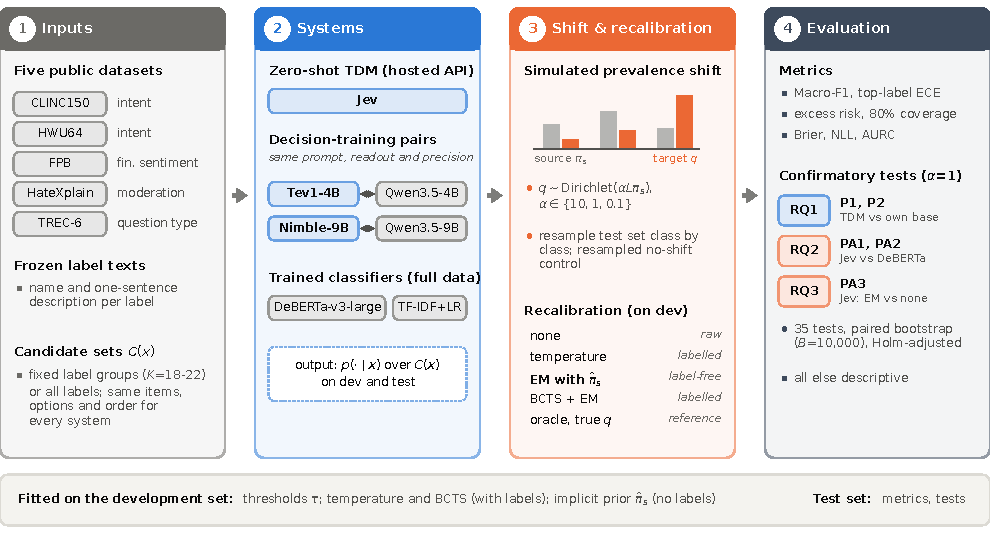
\includegraphics[width=\linewidth]{figures/fig_pipeline.pdf}
  \caption{\textbf{All systems answer identical candidate-set decisions, and shift, recalibration and tests operate on
  their saved probabilities, so every comparison is paired.}
  (1) Five public datasets with frozen label texts and fixed candidate sets. (2) A hosted TDM, two open TDMs each paired
  with its own backbone, and models trained on task labels (two classifiers on the full data and on label budgets, and a
  QLoRA adapter on Qwen3.5-4B) return a probability vector over the candidates. (3) The test set
  is resampled to simulated target priors (\hyperref[eq:shift]{Eq.~\ref*{eq:shift}}), and five recalibration arms are fitted on the unshifted
  development set (\hyperref[eq:implicit]{Eqs.~\ref*{eq:implicit}}--\nobreak\ref{eq:em}). (4) Metrics (\hyperref[eq:ece]{Eqs.~\ref*{eq:ece}} and~\ref{eq:risk}), the 35
  confirmatory tests (\hyperref[eq:pa1]{Eqs.~\ref*{eq:pa1}}--\nobreak\ref{eq:pa3}) and the label-budget curves, which are
  estimated, not tested; everything else is descriptive.}
  \label{fig:pipeline}
\end{figure}

\paragraph{Decision models and candidate sets.}
Let $\mathcal{Y}$ be the label set of a dataset and $L=|\mathcal{Y}|$ its number of classes. Each test example $x$ comes
with a candidate set $C(x)\subseteq\mathcal{Y}$ of $K$ labels that always contains the gold label. A system returns a
probability vector $p(\cdot\mid x)$ over $C(x)$. The prediction is $\hat y=\arg\max_{c\in C(x)} p(c\mid x)$, with ties
broken by candidate position, and the confidence is $\max_{c\in C(x)} p(c\mid x)$. All systems receive the same candidate
set, in the same order, for every example (\hyperref[sec:protocol]{Section~\ref*{sec:protocol}}).

\paragraph{Prevalence shift.}
Let $\pi_s$ be the class distribution of the source data and $q$ that of the deployment data. Under prevalence (label)
shift, $q\neq\pi_s$ while $p(x\mid y)$ is unchanged. We simulate it with a source-centred variant of the Dirichlet shift
of \citet{lipton2018detecting} and \citet{alexandari2020maximum}, who use a symmetric concentration, by drawing a target
prior and class counts for a sample of the test size $n$,
\begin{equation}
  q\sim\mathrm{Dirichlet}(\alpha L\,\pi_s),\qquad (n_y)_{y\in\mathcal{Y}}\mid q\sim\mathrm{Multinomial}(n,q),
  \label{eq:shift}
\end{equation}
where $\pi_s$ is the class distribution of the training split (the same for all systems), and then drawing $n_y$ test
examples of class $y$ with replacement; we call the result the shifted sample $S_q$. The concentration $\alpha L\pi_s$
centres the draws on the source prior and reduces to the usual $\mathrm{Dirichlet}(\alpha\mathbf{1})$ when $\pi_s$ is
uniform. Smaller $\alpha$ means stronger shift; we use $\alpha\in\{10,1,0.1\}$, and the confirmatory tests use $\alpha=1$.

\paragraph{Source prior and implicit prior.}
Prior correction needs the source prior $\pi_s$. For a trained classifier it is the class distribution of its training
data. A zero-shot model has no training data for the task, so we use its \emph{implicit prior}, the smoothed mean
predicted distribution over the $n_{\mathrm{dev}}$ development examples,
\begin{equation}
  \hat\pi_s(y)=\frac{\frac{1}{n_{\mathrm{dev}}}\sum_{i=1}^{n_{\mathrm{dev}}}p(y\mid x_i)+\epsilon}{1+L\epsilon},
  \qquad \epsilon=10^{-3},
  \label{eq:implicit}
\end{equation}
where $p(y\mid x_i)=0$ for $y\notin C(x_i)$; the smoothing keeps classes that the model never predicts from receiving a
prior of zero. This estimate needs no labels. It is motivated by the law of total probability: if the model's posteriors
were calibrated on the source distribution, their mean would equal the source prior, $\mathbb{E}_{x}[p(y\mid
x)]=\pi_s(y)$, and EM started from $\hat\pi_s$ would leave an unshifted sample unchanged. The implicit prior is thus the
source prior with which the model's own posteriors are consistent, a proxy in the spirit of black-box shift estimation
\citep{lipton2018detecting}. The converse does not hold. Agreement of the mean prediction with $\hat\pi_s$ is a property
of the marginal only; it does not make $p(y\mid x)$ the source posterior, which is what the likelihood argument for EM
requires \citep{saerens2002adjusting}. For a miscalibrated model, EM with $\hat\pi_s$ is therefore not a consistent
estimator of the target prior, and we treat it as an empirical, label-free correction whose effect is tested (PA3)
rather than guaranteed. A simulation with deliberately distorted posteriors (exploratory;
\hyperref[tab:emmiscal]{Table~\ref*{tab:emmiscal}}) shows the estimate degrading as calibration worsens, most for
underconfident posteriors, while staying far closer to the target prior than no correction, and with distorted
posteriors the implicit prior serves EM at least as well as the true source prior. EM also only rescales probabilities: a candidate to which the model assigns
probability zero keeps it after correction, so EM cannot repair the examples on which Jev gives the gold label
probability zero (below). Empirically, it is close to the true class distribution on the intent datasets and far from it
on FPB and HateXplain, where the models have a label bias: its total-variation distance to the development set's class distribution is
at most 0.033 for every zero-shot system on CLINC150, but 0.17--0.38 on FPB and 0.23--0.27 on HateXplain
(\hyperref[tab:implicitprior]{Table~\ref*{tab:implicitprior}}; \hyperref[fig:implicitprior]{Figure~\ref*{fig:implicitprior}}). We do not evaluate BBSE or RLLS themselves, because they need a confusion
matrix estimated on labelled data, whereas our question concerns correction without labels; labelled recalibration is
evaluated separately (BCTS+EM).

\paragraph{Recalibration arms.}
For every system we compare five ways of producing probabilities on the shifted test set; the four deployable ones are
fitted on the unshifted development set without target labels, and the oracle uses the true target prior:
\textbf{none} (raw probabilities);
\textbf{temperature} scaling \citep{guo2017calibration};
\textbf{EM} prior correction \citep{saerens2002adjusting};
\textbf{BCTS+EM}, bias-corrected temperature scaling followed by EM \citep{alexandari2020maximum}; and
\textbf{oracle}, prior correction with the true target prior $q$ (an upper reference, not a deployable method).
EM starts from $\hat q^{(0)}=\hat\pi_s$ and alternates, for the $n$ examples of the shifted sample and $y\in C(x)$,
\begin{equation}
  \tilde p^{(t)}(y\mid x)=\frac{p(y\mid x)\,\hat q^{(t)}(y)/\hat\pi_s(y)}
  {\sum_{y'\in C(x)}p(y'\mid x)\,\hat q^{(t)}(y')/\hat\pi_s(y')},\qquad
  \hat q^{(t+1)}(y)=\frac{1}{n}\sum_{i=1}^{n}\tilde p^{(t)}(y\mid x_i),
  \label{eq:em}
\end{equation}
until $\max_y|\hat q^{(t+1)}(y)-\hat q^{(t)}(y)|<10^{-6}$ (at most 100 iterations). The oracle arm applies the E-step
once with $q$ in place of $\hat q^{(t)}$.

\paragraph{EM on candidate sets.}
For CLINC150 and HWU64 the prior lives on all $L$ classes while each posterior is restricted to its candidate set, which
is why the E-step normalises over $C(x)$ only. This is the EM of \citet{saerens2002adjusting} with the pair
$z=(x,C(x))$ as the observation in place of $x$, and it inherits that method's justification if $p(z\mid y)$ is the
same in source and target. That holds in our design: on CLINC150 and HWU64 the candidate set is the fixed group $G(y)$
of the gold label, and on the other datasets it contains every label, so in both cases $C$ is determined by $y$ and
$p(z\mid y)=p(x\mid y)\,\mathbf{1}[C=G(y)]$ is unchanged by a prior shift. The order of the options carries no
information about $y$, because the gold position is counterbalanced (\hyperref[sec:protocol]{Section~\ref*{sec:protocol}}).
Bayes' rule then gives $p_t(y\mid z)\propto p_s(y\mid z)\,q(y)/\pi_s(y)$ for $y\in C(x)$ and zero outside, the E-step of
\hyperref[eq:em]{Eq.~\ref*{eq:em}}, and the M-step is the fixed point of the likelihood of the observed $z$. Two
consequences follow. Because $C(x)$ reveals the group, EM only redistributes probability among the classes of a group:
the estimated mass of each group equals its share of the shifted sample. And the source prior must be the one with which
the posteriors $p_s(y\mid z)$ are consistent, which for a zero-shot model is its implicit prior rather than the training
prior. Our shift simulation resamples whole examples with their candidate sets, so $p(z\mid y)$ is unchanged by
construction. In a deployment, an upstream step would choose the group. If that step is a fixed function of the input,
its choices alone do not break the invariance of $p(z\mid y)$ under label shift; what fails is support: when the chosen
group excludes the gold label, the restricted posterior gives that label probability zero, and no prior correction can
recover it. A simulation with exactly calibrated posteriors (exploratory; \hyperref[tab:emsim]{Table~\ref*{tab:emsim}})
bears this out: with the gold label's group as candidate set, the EM estimate of the target prior is almost as accurate
as the sample's own class shares, and it degrades steadily as a group selector misses the gold label's group more
often.

\paragraph{Metrics.}
Our main calibration metric is top-label expected calibration error with 15 equal-width confidence bins
$B_b=[(b-1)/15,\,b/15)$, the last bin closed \citep{guo2017calibration},
\begin{equation}
  \mathrm{ECE}(S)=\sum_{b=1}^{15}\frac{|B_b|}{|S|}\,\bigl|\mathrm{acc}(B_b)-\mathrm{conf}(B_b)\bigr|,
  \label{eq:ece}
\end{equation}
where $\mathrm{acc}$ and $\mathrm{conf}$ are the accuracy and mean confidence of the examples of $S$ in a bin. Selective
prediction accepts an example if its confidence $c_i$ reaches a threshold $\tau$, chosen on the development set as the
$\lceil 0.8\,n_{\mathrm{dev}}\rceil$-th largest confidence, so that (with ties, at least) 80\% of development examples are
accepted; each recalibration arm has its own threshold. Its selective risk \citep{geifman2017selective} on a sample $S$ and, under
shift, its \emph{excess risk} relative to the unshifted test sample are
\begin{equation}
  R(S;\tau)=\frac{\sum_{i\in S}\mathbf{1}[c_i\ge\tau]\,\mathbf{1}[\hat y_i\neq y_i]}{\sum_{i\in S}\mathbf{1}[c_i\ge\tau]},
  \qquad
  \Delta R(S_q)=R(S_q;\tau)-R(T;\tau),
  \label{eq:risk}
\end{equation}
where $T$ is the unshifted test sample. We also report Macro-F1, accuracy, MCC, Brier score, negative log-likelihood
(NLL, with probabilities clipped at $10^{-12}$, since Jev returns exact zeros) and the area under the risk--coverage
curve (AURC). Jev assigns probability zero to the gold label on 0.4--7\% of test examples (most on HateXplain), so its
NLL is dominated by the clip and is reported for completeness only. Because top-label ECE is biased upward on resampled data, we also report the change in Brier score and NLL
under shift (\hyperref[tab:brier]{Tables~\ref*{tab:brier}} and~\ref{tab:nll}).

\paragraph{Test statistics.}
P1 and P2 compare a TDM with its own base model on the same test examples, $\Delta=m(\mathrm{TDM})-m(\mathrm{base})$ for
$m\in\{\text{Macro-F1},\mathrm{ECE}\}$. PA1--PA3 are defined on a fixed set of $M=50$ target priors $q_1,\dots,q_M$,
drawn once from \hyperref[eq:shift]{Eq.~\ref*{eq:shift}} at $\alpha=1$. For a test sample $T$, let $S_m$ be its shifted sample under $q_m$ and
$N_m$ a no-shift control drawn by the same resampler at $T$'s own class distribution. With $J$ for Jev and $D$ for
DeBERTa-v3-large,
\begin{align}
  \mathrm{PA1}&=\frac{1}{M}\sum_{m=1}^{M}\Bigl(\bigl[\mathrm{ECE}_J(S_m)-\mathrm{ECE}_J(N_m)\bigr]
    -\bigl[\mathrm{ECE}_D(S_m)-\mathrm{ECE}_D(N_m)\bigr]\Bigr),\label{eq:pa1}\\
  \mathrm{PA2}&=\frac{1}{M}\sum_{m=1}^{M}\Bigl(\Delta R_J(S_m)-\Delta R_D(S_m)\Bigr),\label{eq:pa2}\\
  \mathrm{PA3}&=\frac{1}{M}\sum_{m=1}^{M}\Bigl(\mathrm{ECE}^{\mathrm{EM}}_J(S_m)-\mathrm{ECE}_J(S_m)\Bigr),\label{eq:pa3}
\end{align}
where each system uses its own threshold in $\Delta R$ and $\mathrm{ECE}^{\mathrm{EM}}_J$ is computed after EM with
Jev's implicit prior. Positive PA1 and PA2 mean that Jev degrades more than DeBERTa-v3-large under shift; negative PA3
means that EM helps. PA1 subtracts a resampled control because ECE is biased upward on resampled data, whereas PA2 does
not need one because selective risk, a mean of per-example losses over the accepted examples, is nearly unbiased under
resampling. \hyperref[sec:protocol]{Section~\ref*{sec:protocol}} describes how $T$ is
resampled to obtain intervals.

\paragraph{Hypotheses.}
RQ1--RQ3 of \hyperref[sec:intro]{Section~\ref*{sec:intro}} map to the following tests, all specified before the final
test-set runs.
\textbf{H1} (RQ1): vendor decision training changes Macro-F1 or ECE relative to the base model (two-sided). The
controlled test is P2 (Nimble-9B vs Qwen3.5-9B: same base weights and precision, differing only by an adapter). P1
(Tev1-4B vs Qwen3.5-4B) is the closest available comparison, since Tev1 is a full fine-tune whose exact recipe is not
published.
\textbf{H2} (RQ2): under shift, the change in ECE (PA1, \hyperref[eq:pa1]{Eq.~\ref*{eq:pa1}}) and the excess threshold risk (PA2,
\hyperref[eq:pa2]{Eq.~\ref*{eq:pa2}}) differ between Jev and DeBERTa-v3-large (two-sided).
\textbf{H3} (RQ3): EM prior correction with Jev's implicit prior lowers Jev's ECE under shift (PA3, \hyperref[eq:pa3]{Eq.~\ref*{eq:pa3}},
tested two-sided, which is conservative for this directional hypothesis). This confirmatory test concerns plain EM on
Jev only; the other arms and systems are reported descriptively.

\paragraph{Label budgets and crossover.}
RQ4 is answered by estimation, not by a test. For a trained system $s$ with $b$ training labels and seeds
$k=1,\dots,K$, let $\Delta(b)=\frac{1}{K}\sum_{k}m(s_{b,k})-m(J)$ be the paired Macro-F1 difference to Jev on the same
test examples. Its 95\% interval comes from a bootstrap that resamples both the $K$ seeds and the test examples
($B=10{,}000$), so it covers training variation as well as test-set noise. The \emph{crossover budget} is the smallest
evaluated budget $b$ whose interval lies above zero; we report it as the interval between that budget and the one before
it, or as ``not reached'' if no budget up to the full training set qualifies. As a rough guide, we also give the budget
at which the linearly interpolated point estimate first crosses zero \citep{lescao2021howmany}.
